% $Id

%% Dokumentenklasse (Koma Script) -----------------------------------------
\documentclass[%
   %draft,     % Entwurfsstadium
   final,      % fertiges Dokument
	 % --- Paper Settings ---
   paper=a4,% [Todo: add alternatives]
   paper=portrait, % landscape
   pagesize=auto, % driver
   twocolumn,
   % --- Base Font Size ---
   fontsize=10pt,%
	 % --- Koma Script Version ---
   version=last, %
 ]{scrartcl} % Classes: scrartcl, scrreprt, scrbook


% Encoding der Dateien (sonst funktionieren Umlaute nicht)
% Fuer Linux -> utf8
% Fuer Windows, alte Linux Distributionen -> latin1

% Empfohlen latin1, da einige Pakete mit utf8 Zeichen nicht
% funktionieren, z.B: listings, soul.

%\usepackage[latin1]{inputenc}
%\usepackage[ansinew]{inputenc}
\usepackage[utf8]{inputenc}
%\usepackage{ucs}
%\usepackage[utf8x]{inputenc}

\usepackage[T1]{fontenc}
\usepackage[english]{babel}

\addto\captionsenglish{
  \renewcommand{\contentsname}{Table of Contents}
}

\usepackage{multicol}
%\usepackage[scaled]{uarial}


\renewcommand{\rmdefault}{phv} % Arial
\renewcommand{\sfdefault}{phv} % Arial

\usepackage{appendix}
\usepackage{listings}
\usepackage{color}
\usepackage{geometry}
\usepackage{array}
\usepackage{graphicx}
\usepackage{caption}


\usepackage{subcaption}
%prefer subcaption instead of subfigure
%\usepackage{subfigure}

\usepackage{float}
%\usepackage{tikz}
%\usetikzlibrary{arrows}

\usepackage{tikz}
\usetikzlibrary{matrix,calc,shapes}

\tikzset{
  treenode/.style = {shape=rectangle, rounded corners,
                     draw, anchor=center,
                     text width=5em, align=center,
                     top color=white, bottom color=blue!20,
                     inner sep=1ex},
  decision/.style = {treenode, diamond, inner sep=0pt},
  root/.style     = {treenode, font=\Large, bottom color=green!30},
  env/.style      = {treenode, font=\ttfamily\normalsize},
  finish/.style   = {root, bottom color=green!40},
  dummy/.style    = {circle,draw}
}
\newcommand{\yes}{edge node [above] {yes}}
\newcommand{\no}{edge  node [left]  {no}}

%\usepackage{hyperref}

\sffamily

%% Titel -----------------------------------------
\title{Recognition of Human Facial Expressions by Mid-Level Discriminative Patches}
\subtitle{Research Project Master Artificial Intelligence Group 4}
\author{Stefan Selzer I6123079\\Chang Sun I6113630}


%% Dokument -----------------------------------------
\begin{document}

%\begin{@twocolumnfalse}
\onecolumn

\maketitle
\thispagestyle{empty}

\newpage


\begin{abstract}

TODO: same as introduction, change one of them !!
\\
\\
Unsupervised Discovery of mid-level discriminative patches is a method to extract the primitives for visual information from an image.  Singh et al. elaborated on this method by stating that the primitives have to satisfy the requirements of being representative as well as discriminative and having been discovered in a fully unsupervised manner \cite{Singh2012DiscPat}. The method combines techniques from the fields of computer vision and machine learning to produce promising results in image recognition and classification. 
\\
\\
The aim of this project is to apply this method on the classification of images of human facial expressions. This can, for example, aid in human-computer interaction by recognizing particular emotions or cognitive states through visual or expressive features contained in an image. Then computers are enabled to react and interact with the counterpart in an appropriate manner. As a result of the project's work an application has been developed for classification of human emotions and the effectiveness of the image recognition by this classification will be proven with selected, distinct features of various images showing different facial expressions.
\end{abstract}

\thispagestyle{empty}

\newpage
\pagenumbering{roman}
\tableofcontents

\newpage
\listoffigures
\addcontentsline{toc}{section}{List of Figures}
\listoftables
\addcontentsline{toc}{section}{List of Tables}

\newpage
\pagenumbering{arabic}

%\end{@twocolumnfalse}

%\begin{multicols}{2}

\twocolumn



\section{Introduction}\label{sec:Introduction}

TODO: Give an intorduction to the problem and an outline of the work
\\
\\
Unsupervised Discovery of mid-level discriminative patches is a method to extract the primitives for visual information from an image.  Singh et al. elaborated on this method by stating that the primitives have to satisfy the requirements of being representative as well as discriminative and having been discovered in a fully unsupervised manner \cite{Singh2012DiscPat}. The method combines techniques from the fields of computer vision and machine learning to produce promising results in image recognition and classification. 
\\
\\
The aim of this project is to apply this method on the classification of images of human facial expressions. This could, for example, aid in human-computer interaction by recognizing particular emotions or cognitive states through visual or expressive features contained in an image. The purpose of this project is to determine classifiers for human facial expressions by delivering an extensible, easy-to use and well documented code base using C++ as programming language and the image processing library OpenCV as toolset for the basic techniques and algorithms needed to implement the functionality. This paper describes the results of the research project by first giving an overview of the technical background and describing the method implemented by Singh et Al. \cite{Singh2012DiscPat}. Then the project work is presented and finally and outlook on possible future work is given.

\section{Technical Approach}\label{sec:StateArt}

This section gives an explanation of definitions used and an overview of the algorithm proposed by Singh et Al. \cite{Singh2012DiscPat} and the image processing techniques used therein.

\subsection{Definition of Image Patches}

To explain the notion of mid-level discriminative patches, it is best to first observe the different levels of visual information, that can be retrieved from an image. From a bottom-up point-of-view, the lowest level corresponds to a single pixel, but single pixels do obviously not provide much useful information to describe features of the real world. On the opposite side, the highest level corresponds to the image as a whole. This poses several problems on the analysis of the retrieved information such as a high number of spatial configurations needed to describe objects. Also the image as a whole contains too much unnecessary information to describe certain features on their own. As Sing et Al. pointed out \cite{Singh2012DiscPat}, the optimal level of information is found by looking at medium-sized parts of the image, that describe one certain feature of an image. Such parts are called mid-level image patches. Singh et Al. \cite{Singh2012DiscPat} define such patches as being discriminative, if they clearly represent the described feature and if they are different enough from other patches describing the same or any other feature. Additionally, they require such patches to be detectable with "high recall and precision" in a large number of images.

\subsection{Classification of Image Patches}

The algorithm to detect discriminative patches in an unsupervised manner mainly consists of three parts: The first one is to extract features from an image, next these features are clustered and for each cluster a linear support vector machine (SVM) is trained, which is finally used to classify unknown images. In terms of classification of facial expressions, for example, one feature, that distinguishes different emotional expressions, can be the mouth. Happiness is expressed by smiling and showing the teeth, while surprise is usually expressed with a wide open mouth. In this example the mouth parts of an image will be extracted and analyzed. The obtained data from this feature extraction analysis is then used to train SVMs for different emotions, in case of happiness taking the smiling mouths as positive examples and examples from other emotions as negative samples.
\\
\\
Technically, the feature extraction is performed by using the Histogram of Oriented Gradients (HOG) presented by Dalal and Triggs \cite{Dalal:2005:HOG:1068507.1069007}. The features are computed as intensity gradients for small parts of an image. The computed edge directions are then counted and concatenated to form a comprehensive descriptor. One of the key advantages of this technique is, that it is invariant to geometric or photometric transformations. Dalal and Triggs showed \cite{Dalal:2005:HOG:1068507.1069007}, that the HOG features produce good results, when they are used for classification of images. The initial classification step then is performed by clustering the features using k-means clustering. This promising starting point for image classification has been presented by Coates et Al. \cite{DBLP:series/lncs/CoatesN12}. K-means clustering, introduced in \cite{macqueen1967}, partitions a dataset into a given number of clusters in such a way, that the sum of the quadratic deviations from each cluster centroid is minimized. As metric usually the Euclidian distance is used. The actual classification finally is performed by a linear SVM. A linear SVM separates points with a hyperplane, that has a maximized distance to the nearest data points on each side of the plane. This can be used as binary classifier to classify input data according to recognized patterns as shown by Chang et Al. \cite{Chang:2011:LLS:1961189.1961199}. These patterns are obtained by training the SVM on positive and negative samples of data describing the problem, that needs to be solved by classification. The training of the classifier is done one-vs-all. In terms of this project, this means, that the patches extracted for one certain emotion are used as positive samples and an equal number of samples of patches extracted in an evenly distributed manner from all other emotions is used as negative counterpart for the training of the classifiers. The equal number of positive and negative samples ensures a well-balanced classification. Otherwise a larger number of one of the two parts, positive or negative, could influence the outcome of the prediction for validation data in the direction of this larger part.

\subsection{Unsupervised Detection of Discriminative Patches}

Applying these techniques, the feature extraction using HOG descriptors produces a large number of possibly overlapping patches at multiple scales. From these patches, extracted from all over the image, the most discriminative ones have to be obtained automatically. This is done by combining the clustering using k-means and the classification using a linear SVM to refine and enhance each other. Performing this iteratively produces the desired patch clusters containing similar patches, i.e. patches describing the same visual information. 
\\
\\
Initially, this similarity is unknown and has to be discovered. If some of these patches are known to be similar, these similar patches could be used to train a SVM for classification. Fortunately, a similarity can be produced by clustering the patches using k-means clustering. The problem with the low-level metric used by k-means clustering is, that it produces poor results on image patches. To refine the clusters, again, a SVM could be trained to produce a similarity metric. That means, that the clustering depends on the similarity metric of the SVM while the SVM itself depends on the clusters to be trained. To solve this problem, the described approach is performed in an iterative way. First, the data is clustered in HOG space and then a SVM is trained. The SVM uses the clusters to produce a metric which then is used to refine the clusters. This is repeated until a convergence criterion is reached, for example, that the best clusters identified so far do not change anymore. The classifiers found are ranked according to their purity and discriminativeness. Singh et Al. \cite{Singh2012DiscPat} define purity as the sum of the classifiers detection scores of the top cluster members. Discriminativeness describes the ratio of detections on the positive training data and the union of the positive and negative training data. This ratio should be low but still above 0. Finally, the best classifier ranked like this is built upon and identifies the most discriminative patch, that can be found in the original images.

\subsection{Problem of Overfitting}

The drawback of the process described is, that the classifier might suffer from overfitting. Overfitting occurs, for example, when the number of features exceeds the number of training data. In this case, the classifier does not predict by generalizing from what he has learned but memorizes input patterns and recalls them. This effect can be measured by comparing the accuracy of the prediction of training data with the one of unknown validation data. In this case, the prediction of training samples is far more accurate than the prediction of unknown validation data. To prevent this overfitting, the input data of the algorithm can be divided into two datasets initially. One of these two datasets will then act as training data and the other as validation data. In each iteration of the algorithm, the datasets are exchanged for the next iteration to enhance the clusters by new feature patches. This means, the SVM is trained with the training data and the trained classifiers are then used to predict the samples of the validation data. The patches in the validation dataset, that are classified with the best score, will be added to the already obtained clusters to ensure more diversity. This is repeated in the next iteration using the validation data for training and the training data for validation. Overfitting is a particular problem for this project, as on the one hand, the features need a certain minimal amount of detail for the patches to be distinguishable. On the other hand, it is difficult to obtain enough data to train the SVMs, as human facial expressions are retrieved from images of humans. As humans need to explicitly agree 
with the usage of their personal data and additionally the expressions need to be expressive enough, data sets for this kind of problem are few in amount.


\section{Developed Application for Image Classification}\label{sec:application}

This section presents the application that has been developed. The application can be used to train an SVM for each category of a catalog of images or predict images using already trained SVMs. For training, it loads a set of images and trains SVMs for the given categories. The classifiers work on the HOG features extracted from the input images. The steps of the algorithm that performs the image classification are described in a general manner. Details of the implementation can be found in the appendix section \ref{sec:devdoc}.
\\
\\
To train classifiers, the application loads a catalog of images from the file system. At least 2 different categories have to be provided in separate sub folders. The folder names denote the category labels. If it is desired to obtain more data samples to enhance the training of the classifiers, additional images from the horizontally flipped versions of the input images are computed and added to the input data. This doubles the original sample size and eases the problem of overfitting. To improve the quality of the images in regard of the performed feature extraction, histogram equalization is applied to the images as a preprocessing step of the feature extraction. This increases the contrast of the images and produces sharper edges for the edge gradient computation of the feature extractor. The feature extraction is performed using Histogram of Oriented Gradients. The computed features are split into defined parts for training and validation purpose. If there are multiple samples from a similar source contained in the dataset, the separation will make sure that they are not distributed across the training and validation data. For each category, a training and a validation matrix is built each by the corresponding elements of the category itself as positive samples and an equal number of evenly distributed samples from all other corresponding categories as negative samples. The training matrix is used to train a classifier for each category. The validation matrix is used to test and validate the effectiveness of the trained classifier with a large number of unknown samples. Cross validation can be performed by exchanging the training and the validation matrix to enhance the SVMs with additional data. Finally the trained classifiers can be saved to disc for further usage. There will be one classifier for each category. A flow diagram of the application can be found in Figure \ref{figure:flowchart} in Appendix \ref{sec:implem}.

\section{Experiments}
\nocite{Kanade2000CK+}\nocite{Lucey2010CK+}

TODO: describe setup of datasets sued for training and validation.Present results

\subsection{Data}
For training a system to recognize facial expression effectively, the dataset should focus on several main expressions including anger, disgust, fear, happiness, sadness and surprise. Moreover, a proper dataset should be composed of faces with kinds of face shapes, colors, facial and scalp hairs from many participants with different genders, ethnic backgrounds and ages. 
\\
\\
The dataset this paper adopted is from the Cohn-Kanade Facial Expression Database. The dataset refers to eight emotions including anger, contempt, disgust, fear, happiness, sadness, surprise and neutral expression. There are 5105 images from 123 subjects, who ranged in age from 18 to 30 years. Sixty-five percent are female, eight-five percent are Euro-American and fifteen percent are African-American and Asian. They were observed in an observation room equipped with a chair on which to sit and a camera was located directly in front of the subject. Therefore all images have the uniform background and lighting. The images were digitized into 640*480 or 490 pixel arrays with 8-bit precision for grayscale values and are available in png and jpg. 
\\
\\
In the Cohn-Kanade Facial Expression Dataset, subjects performed a series of several facial displays from neutral expressions to peak expressions and images were taken frame by frame. In order to train a powerful system, we chose neutral faces and obvious expressions. That means there is no indistinguishable expression in our dataset. Figure 1 shows some example of the dataset.



\begin{figure}[h!]
\centering
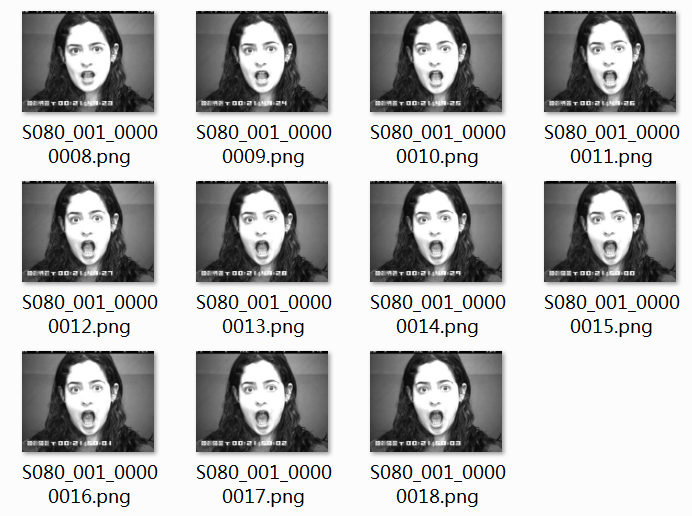
\includegraphics[scale=0.55]{img/example.png}
\caption{Example of dataset}
\label{Example of dataset}
\end{figure}

\subsection{Experiment setup}
The experiments were performed doing one versus all classification. The data for each expression is divided into a training and a validation set and an SVM
classifier is calculated based on the training set. The accuracy of the classifiers is then measured on the validation set. It was ensured that images of the same
person are not present in both the training and validation set. The fraction of the data used for the validation set is a configurable parameter, for the 
following experiments 75\% of the data was used for the training set and 25\% for the valdiation set. 

\subsection{Manual Patches}

An image can have multiple discriminating patches. As shown in Figure \ref{fig:manual_patch}, some patches are highly noticeably discriminating such an open mouth and raised eyebrows in "`surprise"' expression or a wrinkled glabella (area between eyes) in "`disgust"' expression. Such patches can be the best approximation of most discriminating patches. Hence, they make a good basis for testing the algorithm. 

\begin{figure}
\centering
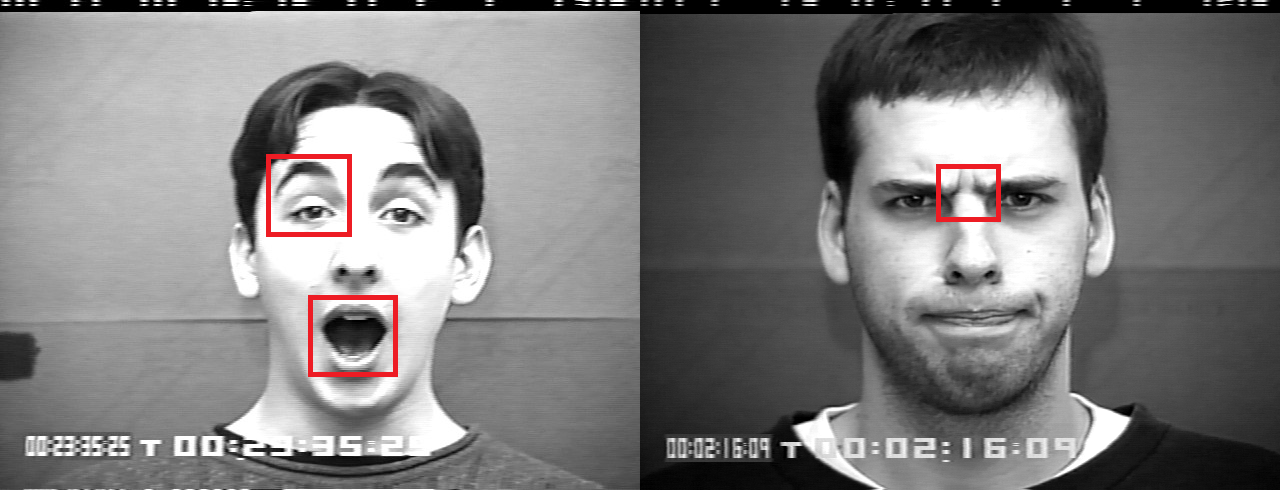
\includegraphics[width=200pt]{img/manual_patch.png}
  \caption{Noticeably discriminating patches}
  \label{fig:manual_patch}
\end{figure}

We identified four such patches, that 2 patches for eyes and one each for mouth and glabella. We extracted them manually and and it was ensured that extracted images of same patch are consistent with each other in terms feature content of the patch. For example, in case of mouth patches, it was ensured that the boundaries of the patch touch the edges of lips in all mouth patches.

Tables \ref{table:left_eye}, \ref{table:right_eye}, \ref{table:between_eyes} and \ref{table:mouth} show the results for each region, for classifiers trained 
with the original patch size of 96x96 and also rescaled to 32x32 and 64x64 pixels. Shrinking the images on the one hand results in fewer hog features which is likely to reduce the effect of  verfitting, on the other hand some visual information may be lost. The table entries represent the fraction of the images of the corresponding expression that were correctly classified, in the 0 to 1 range.



%\subsection{Results}

\begin{table}
\caption{Left eye patches}
\label{table:left_eye}

\begin{tabular}{| c | c | c | c |}
\hline
Expression & 32 x 32 &  64 x 64  & 96 x 96  \\

\hline
Angry & 0.5865 & 0.6786 & 0.7068 \\
Contempt & 0.6596 &	0.5745 & 0.5532 \\
Disgust	& 0.7629 &	0.7629 &	0.7716 \\
Fear &	0.6155 & 0.6315 & 0.6394 \\ 
Happy &	0.6074 & 0.6605 & 0.6529 \\ 
Neutral & 0.6851 &	0.6996 & 0.7093 \\
Sadness & 0.5207 & 0.5041 &	0.5021 \\
Surprise & 0.7652 &	0.7683 & 0.7561 \\

\hline
\end{tabular}
\end{table}

\begin{table}
\caption{Right eye patches}
\label{table:right_eye}

\begin{tabular}{| c | c | c | c |}
\hline
Expression & 32 x 32 &  64 x 64  & 96 x 96  \\

\hline
Angry    & 0.5733 & 0.6466 & 0.6654 \\
Contempt & 0.5638 & 0.5106 & 0.6170 \\ 
Disgust	 & 0.7263 & 0.7414 & 0.7155 \\
Fear	 & 0.6474 & 0.6076 & 0.6096 \\
Happy	 & 0.6367 & 0.6334 & 0.6833 \\
Neutral  & 0.7099 & 0.7272 & 0.7562 \\
Sadness  & 0.5000 & 0.5207 & 0.5456 \\
Surprise & 0.7896 & 0.8171 & 0.8079 \\

\hline
\end{tabular}
\end{table}

\begin{table}
\caption{Part between eyes patches}
\label{table:between_eyes}

\begin{tabular}{| c | c | c | c |}
\hline
Expression & 32 x 32 &  64 x 64  & 96 x 96  \\

\hline
Angry & 0.7971 & 0.812 & 0.7857 \\
Contempt & 0.4468 & 0.4574 & 0.4681 \\
Disgust & 0.6983 & 0.7155 & 0.7306 \\
Fear & 0.7071 & 0.7649 & 0.7351 \\
Happy & 0.8503 & 0.8503 & 0.8329 \\
Neutral & 0.7438 & 0.7845 & 0.7921 \\
Sadness & 0.7324 & 0.7697 & 0.7635 \\
Surprise & 0.7317 & 0.7485 & 0.7165 \\

\hline
\end{tabular}
\end{table}


\begin{table}
\caption{Mouth patches}
\label{table:mouth}

\begin{tabular}{| c | c | c | c |}
\hline
Expression & 32 x 32 &  64 x 64  & 96 x 96  \\

\hline
Angry	&	0.7782	&	0.8064	&	0.7970	\\
Contempt	&	0.6277	&	0.6598	& 0.6702 \\
Disgust	&	0.6918	&	0.7953	&	0.8039	\\
Fear	&	0.7510	&	0.8287	&	0.8307	\\
Happy	&	0.8959	&	0.9121	&	0.9154	\\
Neutral	&	0.7974	&	0.8577	&	0.8501	\\
Sadness	&	0.8589	&	0.8651	&	0.8693	\\
Surprise &	0.8975	&	0.9146	&	0.8959	\\

\hline
\end{tabular}
\end{table}

\subsection{SVM on the entire facial images}
We also experimented with training SVM classifiers considering the entire facial area as a single patch. First the bounding box of the face was detected
for each image using the Viola-Jones algorithm, then rescaled to a uniform size. % TODO: Add Reference. 
The rest of the procedure was identical to the preceding experiment. The results can be found in Table \ref{table:entire_images}.

\begin{table}
\caption{Classifying the whole image}
\label{table:entire_images}

\begin{tabular}{| c | c | c | c |}
\hline
Expression & 32 x 32 &  64 x 64  & 96 x 96  \\

\hline
Angry	 & 0.6165 & 0.6316 & 0.6297	\\
Contempt & 0.4894 & 0.5000 & 0.4043	\\
Disgust	 & 0.7109 & 0.8793 & 0.9367	\\
Fear	 & 0.3540 & 0.6574 & 0.6420	\\
Happy	 & 0.8080 & 0.9317 & 0.9360	\\
Neutral	 & 0.7203 & 0.8260 & 0.8225	\\
Sadness	 & 0.5996 & 0.5830 & 0.6432	\\
Surprise & 0.8765 & 0.9405 & 0.9665	\\

\hline
\end{tabular}
\end{table}

\section{Discussion}
For the manually extracted patches the best overall results were obtained for the mouth region, with over 80\% of the images classified correctly.
This confirms our intuition as this region is the most distinguishable
from a human perspective. Results for the eye regions were better than expected, as visually the extracted patches look very similar. For the disgust emotion all
four regions lead to comparable results, while for the anger emotion the region between the eyes is almost as discriminative as the mouth.
Rescaling the images does not appear to have a very significant effect.
\\
\\
Performing SVM classification on the entire facial region led to good results if the region was rescaled to 96x96 pixels, better than all manually extracted
patches except the mouth. In this case there is a clear loss
of precision if the image is rescaled to 32x32 pixels.
\\
\\
Table \ref{table:predict_series:mouth} shows the result of prediction of mouth patches. Most parts of mouth patches were given correct classifications. However, for angry, fear, happy and surprise emotion, there are one or two ambiguous facial expressions so that the patches of them were classified to an incorrect emotion. By contrast, the prediction of right-eye patches was not as good as that of mouth patches. As Table \ref{table:predict_series:righteye} shows, right-eye patches of angry and fear emotions were not predicted correctly. For other emotions, the accuracy of the prediction of right-eye patches was lower than that of mouth patches.% TODO Run the experiment without face detection to measure the effect, discuss the original paper
\\
\\



\section{Conclusion and Future Work}

The paper described the work and results of the research project on Mid-level Discriminative Patches. An application has been developed making use of parts of the algorithm proposed by Singh et Al. \cite{Singh2012DiscPat} namely the feature extraction using HOG and the classifier using linear SVM. Preprocessing of the data applying histogram equalization ensured good results on the feature extraction. Special care was taken with regard to the setup of the training data in terms of equality in the size of the positive and negative samples and the even distribution of the negative samples among all available negative categories. The acquired data was carefully chosen to contain expressive images to accomplish the task of classifying emotional expressions. Proper separation of the image series in combination with the possibility to add additional images on application runtime ensured the maximum size of training samples available.
\\
\\
From the results of the experiments, it is clear that among all the manually extracted patches, mouth patch is the most representative and distinguishable. The face, as a whole patch, is high-level patch and has too much information. Results of the experiments performed on whole face patches are poorer than mid-level (manually extracted) patches. 
\\
\\
An important component of the algorithm, the k-means clustering, has not been integrated. So fully unsupervised detection has not been achieved. In order to accomplish that, subsets  of the possible patches (memory constraints prohibit loading all of them at once) have to be clustered, and SVM classifiers trained for the largest clusters. New cluster centers can then be calculated using the SVMs as a distance measure. This process can be repeated until the clusters converge, likely resulting in classifiers similar to the ones we've obtained for the manually extracted patches.
\\
\\
The dataset used in this project has subjects with static expressions. That is the subjects were asked to pose for those expressions, which means the expressions were deliberate. For more accurate experimentation a dataset with spontaneous expressions can be used. Cohen et al \cite{cohen2000emotion} discusses some potential extensions and applications of emotional recognition using facial expressions. The algorithm can used to recognize real-time face detection using face tracking. A better and efficient extension can be use of factors such as heart rate and skin conductivity along with face pictures. Emotion recognition can also improvise human-computer interaction. 


\newpage
\appendix
\appendixpage
\addappheadtotoc

\section{User Documentation}\label{sec:userdoc}

The application has three operating modes: train, retrain and predict. In train-mode, new SVMs are trained from given input data. In retrain-mode, already trained SVMs are loaded to enhance them with additional data. In predict-mode, trained SVMs are loaded and used to classify given input data.


\subsection{How to start the application}
The application is implemented as a command line application. It is invoked on the command line by it's name "`MAIProject"' with the filename and path to the configuration file as parameter. The parameter option is denoted as "`-config"'. The following example shows how to call the executable from the current directory assuming the configuration file config.ini is located in the same place.
\begin{verbatim}
./MAIProject -config config.ini
\end{verbatim}

%\lstset{language=bash}
%\begin{lstlisting}
%./MAIProject -config config.ini
%\end{lstlisting}

%\texttt{./MAIProject -config config.ini} 


\subsection{How to configure the application}
The application is configured in detail by a configuration file. This configuration file is formatted using the ini-format. This format follows a simple syntax of key/value pairs noted in one line separated by an equal sign. Sections allow a simple structuring of the key/value pairs. Their names are denoted in square brackets. Section names have to be unique per file and keys have to be unique per section. The file itself is plain text. For this application, there are sections for each part of the implemented algorithm giving detailed control of the configurable aspects of the corresponding feature.
\\
\\
The section MAIN defines the application's operating mode with the parameter MODE. This parameter can have one of the following values: TRAIN, RETRAIN or PREDICT. If the mode set to RETRAIN, the parameter SVM\_FILEPATH defines the location of the already trained SVMs that should be loaded for further training. The data needed for this is configured in the DATA section. In predict-mode, the parameter SVM\_FILEPATH defines the location of the trained SVMs used to classify images. These images are loaded from the location defined in parameter IMAGE\_FILEPATH. This parameter can either define a single image file or a folder containing images. In the latter case, all of the images contained in that folder will be classified.
\\
\\
The section DATA provides parameters to configure the input dataset. The parameter FILEPATH defines the location of the image catalog that should be used for training. The parameter DATASET\_DIVIDER defines the size of the validation part of the input dataset by dividing the size of the whole dataset, e.g. a value of 2 means that 1/2 of the input will be used for validation and 1/2 for training of the SVMs. The flag ADD\_FLIPPED\_IMAGES enables the addition of horizontally flipped versions of the input images to effectively double the overall size of samples, if this is necessary to obtain more training samples.
\\
\\
The section HOG provides parameters to configure the size of image, block and cells, the block stride and the number of bins used to extract the HOG features from the input images. If it is desired to visualize the HOG features together with the image they are computed from, the flag WRITE\_HOGIMAGES can be set together with parameters defining the scaling of the image and the visualized gradients. Concrete values depend on the original image size and the parameters used to compute the features.
\\
\\
The section SVM provides parameters used in combination with the vector machines. The C\_VALUE parameter is used to penalize outliers on an imperfect separation. The flag PREDICT\_TRAININGDATA enables or disables prediction of the dataset used for training. The flag WRITE\_SVM can be set if the trained SVMs should be saved to disc in combination with the parameter FILEPATH, which defines the output location of the saved SVMs. The flag CROSS\_VALIDATE can be set to swap training and validation data and further train the SVMs with the validation data.
\\
\\
The section FACE\_DETECTION provides parameters to configure the haar cascade classifier. The flag DETECT\_FACES enables face detection on the images of the input dataset. The parameter FILENAME defines the path and filename of the trained haar cascade classifier performing the face detection itself. Such classifiers can be found in the corresponding OpenCV package. The parameters MIN\_SIZE and MAX\_SIZE indicate the minimum and maximum possible size of the obtained faces. They depend on the image size of the input dataset which has to be examined to obtain rational values for these parameters.

\section{Developer Documentation}\label{sec:devdoc}


\subsection{Build environment}

The project’s codebase can be configured with CMake \footnote{https://cmake.org/} for development on Linux and Windows. CMake is a platform independent and freely available build tool for C++, that automatically generates compiler configurations. On linux systems, the Makefiles, that are used by the GNU compiler chain, and on Microsoft Windows, Visual Studio project files can be generated from the given configuration. This eliminates the need for tracking such files for different platforms or different versions of development environments.
\\
\\
CMake comes with either command line or GUI tools to configure the concrete setup. The main configuration is defined in the file CMakeLists.txt in the root code folder of the application. Using one of the GUI-tools for configuration for example, the CMakeLists.txt has to be loaded. The configuration then provides variables to set the path to the dependencies. When the configuration is finished, the Makefiles or Visual Studio project files can be generated.


\subsection{Dependencies}

The application has dependencies on OpenCV and the boost c++ libraries. Both libraries have to be installed and added to the system's library path variable. There are non-commercial licenses for both dependencies, so they are freely available and usable without infringement.
\\
\\
OpenCV \footnote{http://opencv.org/} is used in the version 2.4. OpenCV version 3 is not supported, as there are major API changes making it incompatible. The reason for not choosing the latest version was, that this version was released too shortly before the start of this project and has not been in a stable and coherent state at that time regarding the API and the official documentation. OpenCV provides the image processing and machine learning algorithms and techniques used in the application. As it is also configured with CMake, the dependency is configured by simply providing the CMake configuration files of OpenCV, usually located in the root OpenCV installation folder.
\\
\\
The boost c++ libraries \footnote{http://www.boost.org/} are used in the version 1.59.0. As these libraries are downward compatible, later versions can also be used. The boost c++ libraries provide the mechanisms used for file system handling like reading and writing data to and from the file system and for the configuration handling. Though most parts of the libraries are header-only, the file system module requires to either build the libraries or install a complete package containing built libraries. In the CMake configuration, the path to the include files folder and to the installed libraries folder has to be provided to enable the build configuration to set up the Makefiles or Visual Studio project files correctly.


\subsection{Automated HMTL API Documentation Generation}

The application's code contains annotations and comments that can be processed by Doxygen \footnote{http://www.doxygen.org} to automatically generate API documentation in HTML. In combination with the tool "`dot"' from the GraphViz package \footnote{http://www.graphviz.org/}, UML diagrams and flow charts can be generated automatically from the code. A corresponding configuration file is located in the root code folder, called "`Doxyfile"', providing all necessary information to the generator. The generator is invoked from the root code folder as working directory, as the local "`src"' folder is the base for the source files, that have to be processed. Giving the configuration file "`Doxyfile"' as parameter, the generator will put the generated documentation into a local folder called "`doc"'. The "`index.html"' file in the "`doc"' folder is the starting reference for the documentation. An example call from the command line executed in the root code folder of the application looks like this:
\begin{verbatim}
./doxygen Doxyfile
\end{verbatim}


\subsection{Implementation Details}

The data module provides data types and data structures for the application. The class DataSet is the basic data type. It holds the images each together with the file name and the feature vectors extracted from that image. In the course of the main processing pipeline, the images themselves are deleted after the feature extraction step to free memory. The class furthermore provides a method to split the images and respectively their feature vectors into two parts of definable size for training and validation purpose. The class TrainingData holds the training and label matrix needed by the SVM for training in OpenCV matrix format. The constructor creates these matrices from the given vectors of positive and negative training samples, i.e. feature vectors.
\\
\\
The imageCatalog module contains the main application classes for training SVMs on a catalog of images and for classifying images on these trained SVMs. The class CatalogTraining defines the main processing pipeline for training categorized SVMs with a catalog of categorized images. The processing pipeline for single patch images, i.e. manual extracted patches, is setup like this:

\begin{enumerate}
	\item Loading an image catalog from disc.
	\item Refine the images through histogram equalization.
	\item Double the sample size by adding flipped versions (Optional).
	\item Compute the HOG features for the images.
	\item Setup training and validation data.
	\item Train the SVMs on the training data.
	\item Validate the SVMs through prediction of the validation data.
	\item Exchange training and validation data and retrain the SVMs (Optional).
\end{enumerate}

In the course of the process, according methods of the application modules are invoked. The class itself handles the data setup. The class holds a map of categorized DataSets and maps for categorized TrainingData for training and validation purpose. It provides methods to collect positive and negative training samples, from which the TrainingData instances are constructed. These methods ensure equality of the size of positive and negative samples and an even distribution of negative samples among all other categories apart from the current positive one as far as the category sizes permit such equality and even distribution. The class CatalogClassificationSVM holds a map of categorized umSVM instances and provides necessary methods to interact with them. These methods include training the SVMs on the complete catalog of images, loading and saving categorized SVMs, and using the SVM instances for prediction.
\\
\\
The module IOUtils provides static methods for file system handling, input and output of images and basic image operations. There are methods to load a complete catalog of images and methods to load single images or all images contained in a folder. In a catalog of images, the images have to be organized in sub folders according to their categories and the sub folder names define the category names. There are methods to load and save SVMs from and to the file system.
\\
\\
The featureExtraction module provides the functionality for the HOG feature extraction. The class umHOG provides static methods to compute the HOG features for a DataSet object or a single image in OpenCV matrix format. It makes use of the OpenCV HOGDescriptor class to accomplish this task. The feature vectors are of the type vector of floats. The parameters for the extraction process correspond to those needed for the OpenCV HOGDescriptor extraction method. Furthermore the class provides a method to visualize the extracted gradients together with the original image. This method  has been enhanced to support generic input sizes and print out concrete values for gradient average or distinct gradients per extracted cell. The class umPCA provides static methods to reduce the dimensionality of the feature space. It makes use of the OpenCV PCA class and applies the Principal Component Analysis on the cells of the HOG features reducing the dimensionality to the number of gradient bins per cell.
%\footnote{http://www.juergenwiki.de/work/wiki/doku.php?id\=public:hog\_descriptor\_computation\_and\_visualization\#computing\_the\_hog\_descriptor\_using\_opencv}
\\
\\
The svm module provides the functionality for the machine learning parts of the processing pipeline. The class umSVM holds an object of OpenCV CvSVM and provides methods to train this SVM instance, to predict data and load and save this instance. The SVM instance is of type linear SVM C\_SVC, which can be configured using the SVM C value to refine the hyperplane on imperfect separation.
\\
\\
The utils module provides classes for general image processing methods like histogram equalization and adding flipped versions of images. The face detection based on the OpenCV haar cascade classifier is part of this module.
\\
\\
The configuration module provides the classes used for configuring the application. The class Configuration holds the configurable parameters for the application. The parameters are loaded from a given configuration file on instance construction. The class Constants holds the application parameters, that are not supposed to change during normal usage. This includes standard values for the SVM labels and debug flags for debugging the application.

% Bibliography:
%\clearpage
\addcontentsline{toc}{section}{Bibliography}

%\end{multicols}

\bibliographystyle{apalike}
\bibliography{./tex/report}

\section{Project Contributions}

\begin{itemize}
	\item Stefan Selzer
	\begin{itemize}
	\item Complete code development, except for kmeans and part of face detection
	\item Complete thinking, planning and organization
	\item 1/4 of first presentation
	\item Structure, experiments and results for second presentation
	\item Complete Structure, Abstract, Sections 1,2,3 and Appendices of final Report, half of Section 7
	\item Additional data
	\end{itemize}
	\item Chang Sun
	\begin{itemize}
	\item Some small error corrections in the code, part of k-means and face detection.
	\item Data acquisition
	\item 1/4 of first presentation
	\item dataset part of second presentation
	\item Manual patch extraction
	\item Experiments and results for final report
	\item Sections 4.1, 5.3, 5.4, half of section 6
	\end{itemize}
	\item Salil Baht
	\begin{itemize}
	\item 1/4 of first presentation
	\item Manual patch extraction
	\item Section 4.2, half of section 5
	\end{itemize}
	\item Ioannis Papadopoulos
	\begin{itemize}
	\item Some small error corrections in the code, part of k-means.
	\item 1/4 of first presentation
	\item Sections 4.2, 4.4, half of section 6
	\end{itemize}
\end{itemize}


\end{document}
